\chapter{Landasan Teori}
\label{chap:definition}

\section{\textsl{Data Mining}}

\textsl{Data mining} merupakan merupakan proses yang melakukan pengambilan inti sari atau penggalian \textsl{knowledge} dari data yang besar dan merupakan salah satu langkah dari \textsl{knowledge discovery}.


\begin{figure}[H]
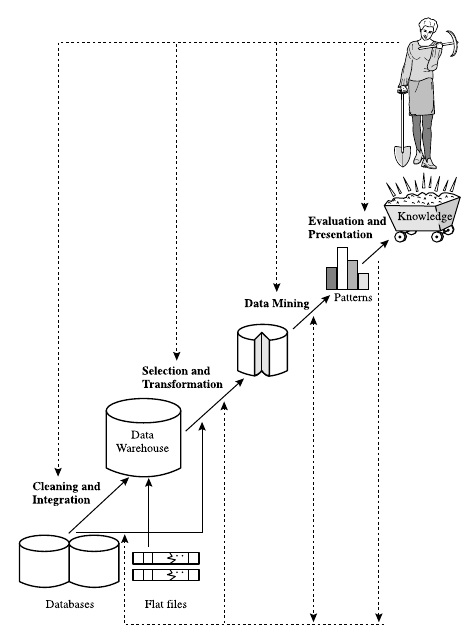
\includegraphics[scale=0.9]{Gambar/tahapdatamining.jpg}
\caption[Tahap \textsl{Data Mining}]{Tahap \textsl{Data Mining}, \cite{DM}} 
\label{fig:tahapDataMining}
\end{figure}

Menurut \cite{DM}, \textsl{knowledge discovery} dapat dibagi menjadi 7 tahap (gambar \ref{fig:tahapDataMining}):
\begin{enumerate}
	\item \textsl{Data cleaning}
	\item \textsl{Data integration}
	\item \textsl{Data selection}
	\item \textsl{Data transformation}
	\item \textsl {Data mining}
	\item \textsl{Pattern Evaluation}
	\item \textsl{Knowledge presentation}
\end{enumerate}


Tahap pertama hingga keempat merupakan bagian dari \textsl{data preprocessing}, dimana data-data disiapkan untuk dilakukan penggalian data. Tahap \textsl{data mining} merupakan tahap dimana melakukan penggalian data. Tahap keenam merupakan tahap pencarian pola yang merepresentasikan \textsl{knowledge}. Sedangkan tahap terakhir merupakan visualisasi dan representasi dari \textsl{knowledge} yang sudah diperoleh dari tahap sebelumnya.


\subsection{\textsl{Data Cleaning}}
\textsl{Data cleaning} merupakan tahap \textsl{data mining} untuk menghilangkan \textsl{missing value} dan \textsl{noisy data}. Pada umumnya, \textsl{data} yang diperoleh dari \textsl{database} terdapat nilai yang tidak sempurna seperti nilai yang hilang, nilai yang tidak valid atau salah ketik. Atribut dari suatu \textsl{database} yang tidak relevan atau redudansi bisa diatasi dengan menghapus atribut tersebut. Contoh studi data yang memiliki \textsl{missing value} dan \textsl{noisy data} dapat dilihat pada tabel \ref{table:contohMissingNNoisy}

\begin{table}[h]
\caption{Tabel mengandung \textsl{missing value} dan \textsl{noisy}}
\label{table:contohMissingNNoisy}
\begin{tabular}{|l|l|l|l|l|}
\hline
IdPenjualan & NamaBarang & Custumer & Harga  & BanyakBarang \\ \hline
1           & Mouse      & Elvin    & 45000  & 2            \\ \hline
2           & Keyboard   & Alleria  & -35000 & 1            \\ \hline
3           & Monitor    &          & 225000 & 1            \\ \hline
\end{tabular}
\end{table}

Dapat dilihat, pada idPenjualan 2, harga dari keyboard adalah -35000, itu merupakan \textsl{noisy} karena tidak mungkin nilai harga suatu barang dibawah 0. Pada idPenjualan 3, kolom \textsl{costumer} tidak memiliki nilai, dan itu merupakan \textsl{missing value}.

\subsubsection{\textsl{Missing Values}}
\textsl{Missing values} akan mengganggu proses \textsl{data mining} pada komputer dan dapat menghasilkan nilai akhir yang tidak sesuai. Terdapat beberapa teknik untuk mengatasi \textsl{missing values} yaitu
	\begin{itemize}
		\item Membuang tuple yang mengandung nilai yang hilang\textit{\textit{}}
		\item Mengisi nilai yang hilang secara manual
		\item Mengisi nilai yang hilang dengan menggunakan nilai konstan yang bersifat umum
		\item Menggunakan nilai rata-rata dari suatu atribut untuk mengisi nilai yang hilang
	\end{itemize}
\subsubsection{\textsl{Noisy Data}}
\textsl{Noisy data} merupakan nilai yang berasal dari error atau tidak valid. \textsl{Noisy data} dapat dihilangkan dengan menggunakan teknik \textsl{smoothing}. Terdapat 3 metode untuk menghilangkan \textsl{noisy data} yaitu
	\label{teknikBinning}
	\begin{itemize}
		\item \textsl{Binning}, merupakan metode pengisian data sesuai dengan proses yang dilakukan pada data tersebut
		\item \textsl{Regression}, merupakan metode yang mencari detail persamaan atribut untuk memprediksikan suatu nilai
		\item	\textsl{Clustering}, merupakan metode pengelompokan dimana ditemukan \textsl{outliers} yang dapat dibuang
	\end{itemize}

%\subsubsection{\textsl{Data Cleaning as a Process}}
%Tahap pertama pada \textsl{data cleaning} adalah \textsl{discrepancy detection}. Ketidakcocokan dapat dikarenakan oleh beberapa faktor, termasuk desain data yang buruk, kesalahan manusia ketika memasukan data, dan data yang sudah kadarluarsa. Ketidakcocokan ini juga dapat disebabkan tidak konsisten representasi data dan kode atau dikarenakan kesalahan perangkat ketika melakukan pemasukan data.

%Untuk mempermudah pencarian ketidakcocokan tersebut, kita dapat membuat sebuah data yang berisi informasi mengenai data atau biasa disebut \textsl{metadata}. Pada tahap ini, penulisan \textsl{script} bisa ditulis dengan cara masing-masing. Disini, dapat ditemukan \textsl{noise}, \textsl{outliers}, dan nilai-nilai yang tidak cocok atau tidak konsisten.

%Data juga harus diperiksa dengan \textsl{unique rules}, \textsl{consecutive rules}, dan \textsl{null rules}. \textsl{unique rules} mengatakan bahwa setiap nilai dari sebuah atribut harus berbeda dengan nilai yang lain pada atribut tersebut. \textsl{Consecutive rules} mengatakan bahwa tidak boleh ada nilai yang hilang diantara nilai tertinggi dan terendah untuk sebuah atribut, dan semua nilai harus bersifat unik. \textsl{null rules} menspesifikasikan penggunaan nilai \textsl{blanks} atau kosong, tanda tanya, karakter spesial, atau \textsl{string} yang dapat menandakan bahwa nilai tersebut bersifat kosong.

%Tahap deteksi ketidakcocokan ini dapat dibantu juga dengan menggunakan \textbf{data scrubbing tools} dan \textbf{data auditing tools}. \textbf{data scrubbing tools} akan menggunakan sebuah domain data untuk melakukan pencarian ketidakcocokan data dan membetulkan data tersebut dengan menggunakan teknik \textsl{parsing} dan \textsl{fuzzy matching}. \textbf{Data auditing tools} akan mencari ketidakcocokan dengan melakukan analisa data untuk menemukan \textsl{rules}, relasi, dan mendeteksi data yang melanggar hal tersebut.

%Beberapa data dapat diperbaiki dengan cara manual, namun sebagian besar data akan membutuhkan \textsl{data transformation} untuk membetulkan data tersebut.

\subsection{\textsl{Data Integration}}
\textsl{Data integration} merupakan tahap menggabungkan data dari berbagai sumber. Sumber tersebut bisa termasuk beberapa \textsl{database}, \textsl{data cubes}, atau bahkan \textsl{flat data}. \textsl{Data cube} merupakan teknik pengambilan data-data dari \textsl{data warehouse} dan dilakukan operasi agregasi sesuai dengan kondisi tertentu (contoh, penjumlahan total penjualan per tahun dari 2005-2010). Sedangkan \textsl{flat data} merupakan data yang disimpan dengan cara apapun untuk merepresentasikan database model pada sebuah data baik berbentuk \textsl{plain text file} maupun \textsl{binary file}. 

Tahap ini harus dilakukan secara teliti terutama ketika dalam memasangkan nilai-nilai yang berasal dari sumber yang berbeda. Pada tahap ini, perlu dilakukan identifikasi data apakah data tersebut dapat diturunkan atau tidak agar data yang diperoleh tidak terlalu besar. \textsl{Data integration} yang baik merupakan integrasi yang dapat memaksimalkan kecepatan dan meningkatkan akurasi dari proses \textsl{data mining}. Contoh studi kasus dari \textsl{data integration}, jika suatu perusahaan sepatu A memiliki dua pabrik dengan \textsl{database} lokal pada masing-masing pabrik, jika akan dilakukan \textsl{data mining} pada kedua \textsl{database }tersebut, maka kedua \textsl{database} akan digabung dan perlu diperhatikan serta diperbaiki nilai-nilai seperti \textsl{primary key}, atribut, dan lain-lain agar tidak terjadi \textsl{error} pada \textsl{database} yang sudah digabung. Proses dari penggabungan hingga perbaikan nilai-nilai pada kedua database tersebut adalah proses \textsl{data integration}.

\subsection{\textsl{Data Selection}}
Proses dimana data-data yang relevan dengan analisis akan diambil dari database dan data yang tidak relevan akan dibuang. Sebagai contoh kasus, jika akan dilakukan analisa mengenai nilai mahasiswa dalam satu semester, atribut pada tabel nilai sebagai berikut
	\begin{itemize}
		\item NPMMahasiswa
		\item NamaMahasiswa
		\item JenisKelamin
		\item Alamat
		\item MataKuliah
		\item NilaiART
		\item NilaiUTS
		\item NilaiUAS
	\end{itemize}
Maka, atribut yang berpotensi diambil adalah MataKuliah, NilaiART, NilaiUTS, NilaiUAS, sedangkan atribut yang akan dibuang adalah NPMMahasiswa, NamaMahasiswa JenisKelamin, dan Alamat karena tidak terlalu berhubungan dengan analisa.

\subsection{\textsl{Data Transformation}}
\textsl{Data transformation} merupakan tahap pengubahan data agar siap dilakukan proses \textsl{data mining}. \textsl{Data transformation} bisa melibatkan:
	\begin{itemize}
		\item \textsl{Smoothing}, proses untuk membuang \textsl{noise} seperti yang dilakukan pada tahap \textsl{data cleaning}
		\item \textsl{Aggregation}, proses mengganti nilai-nilai menjadi suatu nilai yang dapat mewakili nilai sebelumnya
		\item \textsl{Generalization}, proses dimana membuat suatu nilai yang bersifat khusus menjadi nilai yang bersifat umum
		\item \textsl{Normalization}, proses dimana suatu nilai dapat diubah skalanya menjadi nilai yang lebih kecil dan spesifik
		\item \textsl{Attribute construction}, proses membuat atribut baru yang berasal dari beberapa atribut untuk membantu proses data mining
	\end{itemize}
	
\subsubsection{\textsl{Smoothing}}
\textsl{Smoothing} merupakan bagian dari \textsl{data cleaning} untuk menghilangkan \textsl{noise} pada database. Teknik dari \textsl{smoothing} adalah \textsl{binning}, \textsl{regression}, dan \textsl{clustering}. Penjelasan teknik \textsl{smoothing} dapat dilihat pada \ref{teknikBinning}, bagian \textsl{noisy data}.

\subsubsection{\textsl{Aggregation}}
\textsl{Aggregation}, dimana suatu kesimpulan atau hasil dari \textsl{aggregation operation} yang disimpan dalam database. Contoh studi kasus, jika terdapat suatu database dari toko A, kita dapat menggunakan operasi \textsl{aggregation} untuk mencari total pendapatan dengan rentang hari tertentu.

\subsubsection{\textsl{Generalization}}	
\textsl{generalization}, dimana suatu data yang memiliki nilai \textsl{primitive} atau \textsl{low level} diubah menjadi \textsl{high level} dengan menggunakan konsep hirarki. Contoh studi kasus, nilai pada atribut umur dapat dikelompokkan menjadi muda, dewasa, tua.	
	
\subsubsection{\textsl{Normalization}}
Atribut dapat dinormalisasi dengan memberi skala pada nilainya sehingga nilai tersebut menjadi suatu range yang lebih spesifik dan kecil seperti 0,0 sampai 1,0.
Dua teknik nnormalisasi yaitu, \textsl{min-max normalization} dan \textsl{z-score normalization}. \textsl{Min-max normalization} akan mengubah semua nilai menjadi nilai dengan skala tertentu. Dengan menggunakan rumus 

\begin{displaymath}
	\nu' = \frac{\nu-min_{A}}{max_{A}-min_{A}}(newMax_{A}-newMin_{A})+newMin_{A}	
\end{displaymath}

Contoh kasus, misalkan nilai minimun dan maximum dari suatu pendapatan adalah 12.000 dan 98.000, akan diubah menjadi berskala antara 0,0 sampai 1,0. Jika ada nilai pendapat yang baru, yaitu 73.600, maka akan menjadi

\begin{displaymath}
\frac{73.600-12.000}{98.000-12.000} (1,0-0)+0 = 0,716
\end{displaymath}

\textsl{z-score normalization} merupakan normalisasi berdasarkan nilai rata-rata dan standar deviasi dari nilai-nilai atribut dengan cara

\begin{displaymath}
\nu' = \frac{\nu-\overline{A}}{\sigma_{A}}
\end{displaymath}

Contoh kasus, misal nilai rata-rata dan standar deviasi dari nilai-nilai atribut pendapatan adalah 54.000 dan 16.000. Dengan \textsl{z-score}, jika ada nilai pendapatan baru yaitu 73600, maka akan diubah menjadi

\begin{displaymath}
\frac{73.600-54.000}{16.000} = 1,225 
\end{displaymath}

\subsubsection{\textsl{Attribute Construction}}
\textsl{Attribute Construction} merupakan teknik menambahkan atribut baru yang berdasarkan dari atribut yang sudah ada guna menambah akurasi. Contoh kasus, dibuat atribut baru bernama area berdasarkan atribut panjang dan lebar. 

%\subsubsection{\textsl{Data Reduction}}
%Proses \textsl{aggregation} dan \textsl{generalization} akan dilakukan dalam bentuk proses \textsl{data reduction} dan \textsl{Data Cube Aggregation}.
%\textsl{Data reduction} dan dilakukan untuk mendapatkan nilai yang representif namun tetap menjaga keakuratan hasil \textsl{data mining}. Terdapat beberapa cara dalam mengimplementasikan \textsl{data reduction} yaitu
%	\begin{itemize}
%		\item \textsl{Data subset selection}
%		\item \textsl{Dimensionality reduction}
%		\item \textsl{Numerosity reduction}
%		\item \textsl{Discretization and concept hierarchy generation}
%	\end{itemize}	

%\subsubsection {\textsl{Attribute Subset Selection}}
%\textsl{Attribute subset selection} merupakan salah satu cara melakukan \textsl{data reduction} dengan menghilangkan atribut-atribut yang tidak relevan atau data yang redudansi. Hal ini dapat mempermudah pencarian pola dikarenakan atribut yang tidak relevan tidak ada. Tujuan dari \textsl{attribute subset selection} adalah memperoleh set data yang paling sedikit yang tetap menghasilkan probabilitas penyebaran data kelas tetap mirip dengan set data sebelum dikurangi atributnya. 
%Contoh studi kasus, jika toko CD ingin mencari apakah para konsumen tertarik dan membeli CD baru, maka atribut nama dan nomor telepon dari data konsumen tidak terlalu relevan dengan tujuan \textsl{mining} pada kasus ini, sedangkan jenis\_kelamin dan musik\_kesukaan dari konsumen bisa menjadi atribut yang relevan. 

%\subsubsection {\textsl{Dimensionality Reduction}}
%\textsl{Dimensionality Reduction} merupakan metode pengurangan nilai secara acak dengan cara melakukan konversi data. Jika data original dapat dibuat ulang dari data yang sudah dikompresi tanpa kehilangan informasi, maka akan dikatakan \textsl{lossless}, namun jika hanya mendapatkan data pendekatannya saja, akan disebut lossly \cite{DM}.

%\subsubsection {\textsl{Numerosity Reduction}}
%\textsl{Numerosity Reduction} merupakan metode dimana data diganti atau ditentukan dengan cara parametik atau nonparametrik.

%\subsubsection {\textsl{Discretization and Concept Hierarchy Generation}}
%lewat dulu

\subsection{\textsl{Data Mining}}

Pada tahap ini, akan dilakukan proses \textsl{data mining} dengan menggunakan input data yang sudah diproses pada tahap sebelumnya (\textsl{data cleaning, data selection, data integration,} dan /\textsl{data transformation}).

\subsubsection{\textsl{Classification and Prediction}}
\textsl{Classification} merupakan pemodelan yang dibangun untuk memprediksikan label kategori, seperti "`baik"', "`cukup"', dan "`buruk"' dalam sistem penilaian sikap seorang siswa atau "`mini bus"', "`bus"', atau "`sedan"' dalam kategori tipe mobil. Kategori tersebut dapat direpresentasikan dengan menggunakan nilai diskret. Nilai diskret merupakan nilai yang terpisah dan berbeda, seperti 1 atau 5. Kategori yang direpresentasikan oleh nilai diskret maka akan menjadi nilai yang terurut dan tidak memiliki arti, seperti 1,2,3 untuk merepresentasikan kategori tipe mobil "`mini bus"', "`bus"', dan "`sedan"'.

\textsl{Prediction} merupakan model yang dibangun untuk meramalkan fungsi nilai kontinu atau \textsl{ordered value}. \textsl{Ordered value} merupakan nilai yang terurut dan berlanjut. Contoh studi kasus untuk pemodelan prediction adalah seorang marketing ingin meramalkan seberapa banyak konsumen yang akan belanja di sebuah toko dalam waktu satu bulan. Pemodelan tersebut disebut \textsl{predictor}. \textsl{Regression Analysis}, merupakan metodologi statistik yang digunakan untuk \textsl{numeric prediction}. \textsl{Classification} dan \textsl{numeric prediction} merupakan dua jenis utama dalam masalah prediksi.

\textsl{Data Classification} merupakan proses untuk melakukan klasifikasi. \textsl{Data classification} memiliki dua tahap proses, yaitu \textsl{learning step} dan tahap klasifikasi seperti pada ilustrasi di gambar \ref{fig:tahapDataClassification}. \textsl{Learning step} merupakan langkah pembelajaran, di mana algoritma klasifikasi membangun \textsl{classification rules} (yang berisi syarat atau aturan sebuah nilai masuk ke dalam kategori tertentu) dengan cara menganalisis \textsl{training set} yang merupakan \textsl{database tuple}. Karena pembuatan \textsl{classification rules} menggunakan \textsl{training set}, yang dikenal juga sebagai \textsl{supervised learning}. 
Pada tahap kedua, dilakukan proses klasifikasi nilai berdasarkan \textsl{classification rules} yang sudah dibangun dari tahap pertama.

\begin{figure}
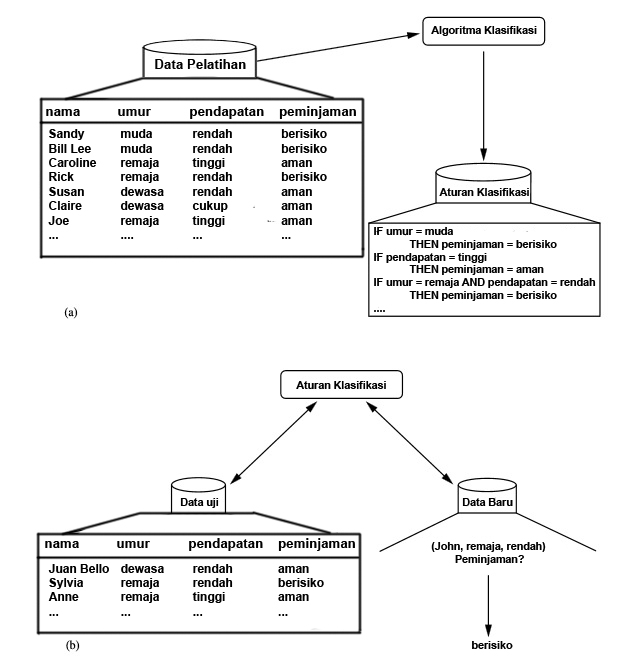
\includegraphics[scale=1]{Gambar/tahapdataclassification.jpg}
\caption[Tahap \textsl{data classification}]{Tahap \textsl{data classification}, \cite{DM}} 
\label{fig:tahapDataClassification}
\end{figure}

\subsubsection{\textsl{Decision Tree}}
Salah satu cara pembuatan \textsl{classification rules} pada \textsl{Data Classification} adalah dengan membuat \textsl{decision tree} (pohon keputusan). \textsl{Decision tree} merupakan \textsl{flowchart} yang berbentuk pohon, dimana setiap node internal (\textsl{nonleaf} node) merupakan hasil test dari atribut, setiap cabang merepresentasikan output dari test, dan setiap node daun memiliki \textsl{class label}. Bagian paling atas dari pohon disebut \textsl{root node}. Contoh studi kasus, pohon keputusan untuk menentukan apakah seorang konsumen akan membeli komputer atau tidak (ilustrasi pohon keputusan pada gambar \ref{fig:decisionTree}) 

\begin{figure}
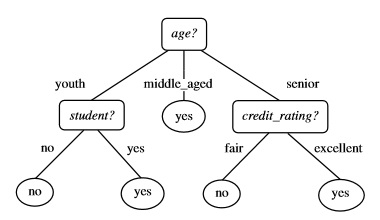
\includegraphics[scale=1]{Gambar/decisiontree.jpg}
\caption[Contoh \textsl{decision tree}]{Contoh \textsl{decision tree}, \cite{DM}} 
\label{fig:decisionTree}
\end{figure}

\paragraph{\textsl{Decision Tree Induction}}

\textsl{Decision tree induction} merupakan pelatihan pohon keputusan dari tupel pelatihan kelas berlabel. Terdapat beberapa teknik untuk membuat \textsl{decission tree} dua diantaranya adalah ID3 dan C4.5. ID3 merupakan teknik pembuatan \textsl{decision tree} dengan memanfaatkan \textsl{entropy} dan \textsl{gain info} untuk menentukan atribut yang terbaik untuk node pada \textsl{decision tree}. Sedangkan C4.5 merupakan teknik lanjutan dari ID3 yang menggunakan \textsl{gain ratio} untuk melakukan pengecekan pada nilai \textsl{gain info}.Kedua teknik tersebut menggunakan pendekatan \textsl{greedy} yang merupakan \textsl{decission tree} yang dibangun secara \textsl{top-down recursive divide and conquer}. Algoritma yang diperlukan secara umum sama, hanya berbeda pada \textsl{attribute\_selection\_method}. Berikut algoritma untuk membuat pohon keputusan dari suatu tupel pelatihan.

Input:
\begin{itemize}
	\item Partisi data, D, merupakan set data pelatihan dan kelas label
	\item \textsl{attribute\_list}, merupakan set dari atribut kandidat
	\item \textsl{Attribute\_selection\_method}, prosedur untuk menentukan \textsl{splitting criterion}. Pada input ini, terdapat juga data \textsl{splitting\_attribute} dan mungkin salah satu dari \textsl{split point} atau \textsl{splitting subset}
\end{itemize}

Output: pohon keputusan
\label{method_pohon_keputusan}
Method:

(1) create a node N;

(2) if tuples in D are all of the same class, C then

(3)	return N as a leaf node labeled with the class C;

(4)	if attribute\_list is empty then

(5) return N as leaf node labeled with the majority class in D; //majority voting

(6)	apply Attribute\_selection\_method(D, atribute\_list) to find the "`best"' splitting\_criterion;

(7) label node N with splitting\_criterion;

(8) if splitting\_attribute is discrete valued and
				multiway splits allowed then //not restricted to binary trees

(9) attribute\_list <- attribute\_list - splitting\_attribute; //remove splitting\_attribute

(10)for each outcome j of splitting\_criterion // partition the tuples and from subtrees for each partition

(11)let D\lowercase{j} be the set of data tuples in D satisfying outcome j; //a partition

(12) if D\lowercase{j} is empty then

(13) attach a leaf labeled with the majority class in D to node N;

(14) else attach the node returned by generate\_decision\_tree(D\lowercase{j}, attribute\_list) to node N;

endfor

(15) return N;

Pohon keputusan akan dimulai dengan satu node, yaitu N, merepresentasikan tuple pelatihan pada D (langkah 1)

Jika tuple di D memiliki kelas yang sama semua, maka node N akan menjadi daun dan diberi label dari kelas tersebut (langkah 2 dan 3). Perlu diketahui bahwa langkah 4 dan 5 akan mengakhiri kondisi.

Jika tuple di D ada kelas yang berbeda, maka algoritma akan memanggil \textsl{attribute\_selection\_method} untuk menentukan \textsl{splitting criterion}. \textsl{Splitting criterion} akan menentukan atribut pada node N yang merupakan nilai terbaik untuk memecah nilai atribut pada tuple ke dalam kelas masing-masing. (langkah 6)

Node N akan diisi dengan hasil dari \textsl{splitting criterion} (langkah 7). Kemudian kriteria tersebut agak dibentuk cabangnya masing-masing sesuai pada langkah 10 dan 11. Terdapat tiga kemungkinan bentuk kriteria jika A merupakan \textsl{splitting\_attribute} yang memiliki nilai unik seperti \{a$_{1}$, a$_{2}$, ..., a$_{v}$\} seperti pada gambar \ref{fig:splitPoint}, yaitu,

\begin{enumerate}
	\item \textsl{Discrete valued}: cabang yang dihasilkan memiliki kelas dengan nilai diskret. Karena kelas yang dihasilkan diskret dan hanya memiliki nilai yang sama pada cabang tersebut, maka \textsl{attribut\_list} akan dihapus (langkah 8 dan 9)
	\item \textsl{Continuous values}: cabang yang dihasilkan memiliki jarak nilai untuk memenuhi suatu kondisi (contoh: A <= split\_point), dimana nilai \textsl{split\_point} adalah nilai pembagi yang dikembalikan oleh \textsl{attribute\_selection\_method}
	\item \textsl{Dicrete valued and a binary tree}: cabang yang dihasilkan adalah dua berupa nilai iya atau tidak dari "`apakah A anggota S$_{a}$"', dimana S$_{a}$ merupakan subset dari A, yang dikembalikan oleh \textsl{Attribute\_selection\_method}
\end{enumerate}


\begin{figure}
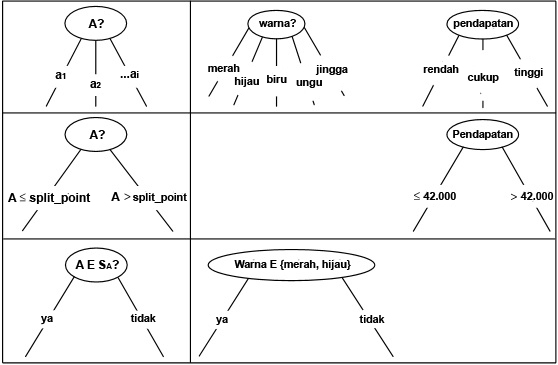
\includegraphics[scale=1]{Gambar/jenishasilsplitpoint.jpg}
\caption[Jenis-jenis \textsl{split point}]{Jenis-jenis \textsl{split point}, \cite{DM}} 
\label{fig:splitPoint}
\end{figure}

Kemudian, akan dipanggil kembali algoritma \textsl{decision tree} untuk setiap nilai hasil pembagian pada tuple, D$_{j}$  (langkah 14).

Rekursif tersebut akan berhenti ketika salah satu dari kondisi terpenuhi, yaitu

\begin{enumerate}
	\item Semua tuple pada partisi D merupakan bagian dari kelas yang sama.
	\item Sudah tidak ada atribut yang dapat dilakukan pembagian lagi (dilakukan pengecekan pada langkah 4). Disini, akan dilakukan \textsl{majority voting} (langkah 5) yang akan mengkonversi node N menjadi \textsl{leaf} dan diberi label dengan kelas yang terbanyak pada D.
	\item Sudah tidak ada tuple yang dapat diberi cabang, D$_{j}$ sudah kosong (langkah 12) dan \textsl{leaf} akan dibuat dengan \textsl{majority class} pada D (langkah 13).
\end{enumerate}

Pada langkah 15, akan dikembalikan nilai \textsl{decision tree} yang telah dibuat.

subsubsection{\textsl{Attribute Selection Measure}}

\textsl{Attribute Selection Measure} merupakan suatu hirarki untuk pemilihan \textsl{splitting criterion} yang terbaik yang memisah partisi data (D), tuple pelatihan kelas label ke dalam kelas masing-masing. \textsl{Attribute Selection Measure} menyediakan peringkat untuk setiap atribut pada training tuple. Jika \textsl{splitting criterion} merupakan nilai \textsl{continous} atau \textsl{binary trees}, maka nilai \textsl{split point} dan \textsl{splitting subset} harus ditentukan sebagai bagian dari \textsl{splitting criterion}. Contoh dari \textsl{attribute selection measure} adalah \textsl{information gain}, \textsl{gain ratio}, dan \textsl{gini index}.

Notasi yang digunakan adalah sebagai berikut. D merupakan data partisi, set pelatihan dari \textsl{class-labeled} tuple. Jika label kelas atribut memiliki m nilai yang berbeda yang mendifinisikan m kelas yang berbeda, $C_{i}$ (for i=1,...,m). C$_{i,d}$ menjadi kelas tuple dari C$_{i}$ di D. |D| dan |C$_{i,d}$| merupakan banyak tuple pada D dan C$_{i,d}$.

\paragraph{\textsl{Information Gain}}

\textsl{Information} menurut Claude Shannon dalam \textsl{information theory} adalah ukuran \textsl{pure} dari suatu data. Suatu data yang \textsl{pure} jika data tersebut memiliki tuple dengan \textsl{class} yang sama. ID3 menggunakan \textsl{information gain} sebagai \textsl{attribute selection measure} yang melakukan pemilihan atribut berdasarkan informasi yang terkandung dalam pesan. Cara ID3 mendapatkan \textsl{information gain} dengan menggunakan \textsl{entropy}. \textsl{Entropy} adalah ukuran \textsl{impurity} dari suatu data. Cara mendapatkan nilai \textsl{entropy} adalah

\begin{displaymath}
	Info(D) = -\sum_{i=1}^{m} pi \log_2(pi)
\end{displaymath}

Dimana pi merupakan probabilitas tuple pada D terhadap class C$_{i}$, dapat diperoleh dengan |C$_{i,d}$|/|D|. Info(D) merupakan nilai rata-rata \textsl{entropy} dari suatu label kelas pada tuple D. Untuk mengetahui atribut mana yang paling baik untuk dijadikan \textsl{splitting attribute}, adalah dengan cara menghitung nilai \textsl{entrophy} dari suatu atribut kemudian diselisihkan dengan nilai \textsl{entropy} dari D. Jika pada tuple D, memiliki atribut A dengan v nilai yang berbeda, maka menghitung \textsl{entropy} dari suatu atribut adalah

\begin{displaymath}
	Info_A(D) = \sum_{j=1}^v \frac{|D_j|}{|D|} \times Info(D_j)
\end{displaymath}

|D$_{j}$|/D merupakan angka yang menghitung bobot dari suatu partisi. Semakin kecil nilai dari Info$_{A}(D)$, maka atribut tersebut masih memerlukan informasi, semakin besar nilai Info$_{A}$(D), semakin tinggi pula tingkat \textsl{pure} dari suatu partisi.

Setelah mendapatkan nilai Info(D) dan Info$_{A}$(D), \textsl{information gain} dapat diperoleh dari selisih nilai Info(D) dan Info$_{A}$(D)

\begin{displaymath}
	Gain(A) = Info(D) - Info_A(D)
\end{displaymath}

contoh kasus untuk ID3, dalam pencarian\textsl{information gain}

\begin{table}[h]
\caption{Contoh training set}
\label{table:contohTrainingSet}
\begin{tabular}{|l|l|l|l|l|l|}
\hline
RID & age          & income & student & credit\_rating & Class: buys\_computer \\ \hline
1   & youth        & high   & no      & fair           & no                    \\ \hline
2   & youth        & high   & no      & excellent      & no                    \\ \hline
3   & middle\_aged & high   & no      & fair           & yes                   \\ \hline
4   & senior       & medium & no      & fair           & yes                   \\ \hline
5   & senior       & low    & yes     & fair           & yes                   \\ \hline
6   & senior       & low    & yes     & excellent      & no                    \\ \hline
7   & middle\_aged & low    & yes     & excellent      & yes                   \\ \hline
8   & youth        & medium & no      & fair           & no                    \\ \hline
9   & youth        & low    & yes     & fair           & yes                   \\ \hline
10  & senior       & medium & yes     & fair           & yes                   \\ \hline
11  & youth        & medium & yes     & excellent      & yes                   \\ \hline
12  & middle\_aged & medium & no      & excellent      & yes                   \\ \hline
13  & middle\_aged & high   & yes     & fair           & yes                   \\ \hline
14  & senior       & medium & no      & excellent      & no                    \\ \hline
\end{tabular}
\end{table}

Pada tabel \ref{table:contohTrainingSet}, terdapat \textsl{training set}, D. Atribut kelas label merupakan dua nilai yang berbeda yaitu \textsl{yes} atau \textsl{no}, maka dari itu, nilai m = 2. C$_{1}$ diisi dengan kelas label bernilai \textsl{yes}, sedangkan C$_{2}$ diisi dengan kelas label bernilai \textsl{no}. Terdapat sembilan tuple atribut kelas label dengan nilai \textsl{yes} dan lima tuple dengan nilai \textsl{no}. Untuk dapat menentukan \textsl{splitting criterion}, \textsl{information gain} harus dihitung untuk setiap atribut terlebih dahulu. Perhitungan \textsl{entropy} untuk D adalah

\begin{displaymath}
	Info(D) = - \frac{9}{14}\log2(\frac{9}{14}) - \frac{5}{14}\log_2(\frac{5}{14}) = 0.940 bits
\end{displaymath}

Setelah diperoleh nilai \textsl{entropy} dari D, kemudian akan dihitung nilai \textsl{entropy} atribut dimulai dari atribut age. Pada kategori \textsl{youth}, terdapat dua tuple dengan kelas \textsl{yes} dan tiga tuple dengan kelas \textsl{no}. Untuk kategori \textsl{middle\_age}, terdapat empat tuple dengan kelas \textsl{yes} dan nol tuple dengan kelas \textsl{no}. Pada kategori \textsl{senior}, terdapat tiga dengan kelas \textsl{yes} dan dua dengan kelas \textsl{no}. Perhitungan nilai \textsl{entropy} atribut \textsl{age} terhadap D sebagai berikut

\begin{displaymath}
	Info_{age}(D) = \frac{5}{14} \times (-\frac{2}{5}\log_2\frac{2}{5} - \frac{3}{5}\log_2\frac{3}{5}) + \frac{4}{14} \times (-\frac{4}{4}\log_2\frac{4}{4} - \frac{0}{4}\log_2\frac{0}{4}) + \frac{5}{14} \times (-\frac{3}{5}\log_2\frac{3}{5} - \frac{2}{5}\log_2\frac{2}{5}) = 0.694 bits
\end{displaymath}

Setelah mendapatkan \textsl{entropy} dari atribut \textsl{age}, maka nilai \textsl{gain information} dari atribut \textsl{age} adalah

\begin{displaymath}
	Gain_{(age)} = Info(D) - Info_{age}(D) = 0.940 - 0.694 = 0.246 bits
\end{displaymath}

Dengan melakukan hal yang sama, dapat diperoleh nilai \textsl{gain} untuk atribut \textsl{income} adalah 0.029 \textsl{bits}, untuk nilai \textsl{gain(student)} adalah 0.151 \textsl{bits}, dan \textsl{gain(credit\_rating)} = 0.048 \textsl{bits}. Karena nilai \textsl{gain} dari atribut \textsl{age} merupakan nilai terbesar diantara semua atribut, maka atribut \textsl{age} dipilih menjadi \textsl{splitting attribute}. Setelah ditentukan, node N akan membentuk cabang berdasarkan nilai dari atribut \textsl{age} seperti pada gambar \ref{fig:hasilCabang}.

\begin{figure}
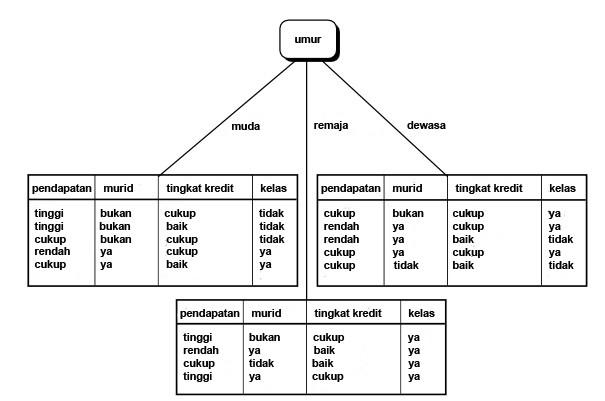
\includegraphics[scale=1]{Gambar/hasilcabangid3.jpg}
\caption[Hasil pohon faktor pada atribut \textsl{age} dari table 2.1]{Hasil cabang dari atribut \textsl{age}, \cite{DM}} 
\label{fig:hasilCabang}
\end{figure}

Untuk atribut yang merupakan nilai \textsl{continuous}, harus dicari nilai \textsl{split point} untuk A. Nilai-nilai dari dua angka yang bersebelahan dapat diambil nilai tengahnya untuk dijadikan \textsl{split-point}. Jika terdapat v nilai yang berbeda dari A, maka akan terdapat v-1 kemungkinan \textsl{split point}. Kemudian nilai \textsl{split point} akan dijadikan sebagai nilai pembagi, sebagai contoh: A <= \textsl{split-point} merupakan cabang pertama, dan A > \textsl{split-point} merupakan cabang kedua.

\paragraph{\textsl{Gain Ratio}}

\textsl{Information gain} akan memiliki nilai yang baik jika suatu atribut memiliki banyak nilai yang berbeda, namun hal itu tidak selalu bagus. Sebagai contoh kasus, jika nilai id suatu table yang memiliki nilai unik, maka akan terdapat banyak sekali cabang. Namun setiap cabang hanya akan berisi satu tuple dan bersifat \textsl{pure}, maka nilai \textsl{entropy} yang dihasilkan adalah 0. Oleh karena itu, informasi yang diperoleh pada atribut ini akan bernilai maksimum namun tidak akan berguna untuk \textsl{classification} \cite{DM}.

C4.5, menggunakan nilai tambahan dari \textsl{information gain} yaitu \textsl{gain ratio}, yang dapat mengatasi permasalahan \textsl{information gain} tentang nilai yang banyak namun tidak baik untuk \textsl{classification}. C4.5 melakukan teknik normalisasi terhadap \textsl{gain information} dengan menggunakan \textsl{split information} yang memiliki rumus sebagai berikut:

\begin{displaymath}
	SplitInfo_A(D) = - \sum_{j=1}^v \frac{|D_j|}{|D|} \times \log_2 (\frac{|D_j|}{|D|})
\end{displaymath}

Setelah mendapatkan nilai \textsl{split info} dari suatu atribut, dapat diperoleh nilai \textsl{gain ratio} dengan rumus sebagai berikut:

\begin{displaymath}
	GainRatio(A) = \frac{Gain(A)}{SplitInfo(A)}
\end{displaymath}

Nilai dari \textsl{gain ratio} terbesar yang akan dipilih. Perlu diketahui \cite{DM} jika nilai hasil mendekati 0, maka ratio menjadi tidak stabil, oleh karena itu, \textsl{gain information} yang dipilih harus besar, minimal sama besarnya dengan nilai rata-rata dari semua test yang diperiksa.

Contoh studi kasus, akan dilakukan perhitungan \textsl{gain ratio} dengan menggunakan training set pada tabel \ref{table:contohTrainingSet}. Dapat dilihat pada atribut \textsl{income} memiliki tiga partisi yaitu \textsl{low}, \textsl{medium}, dan \textsl{high}. Terdapat empat tuple dengan nilai \textsl{low}, enam tuple dengan nilai \textsl{medium}, dan empat tuple dengan nilai \textsl{high}. Untuk menghitung \textsl{gain ratio}, perlu dihitung nilai \textsl{split information} terlebih dahulu dengan cara:

\begin{displaymath}
	SplitInfo_A(D) = - \frac{4}{14} \times \log_2 (\frac{4}{14}) - \frac{6}{14} \times \log_2 (\frac{6}{14}) - \frac{4}{14} \times \log_2 (\frac{4}{14})
	SplitInfo_A(D) = 0.926 bits
\end{displaymath} 

Jika nilai \textsl{gain information} dari \textsl{income} adalah 0.029, maka, dapat diperoleh \textsl{gain ratio} dari \textsl{income} adalah

\begin{displaymath}
	GainRatio(D) = \frac{0.029}{0.926} = 0.031 bits
\end{displaymath}

\paragraph{Tree Pruning}
	
\textsl{Tree pruning} merupakan proses pemotongan \textsl{decision tree} agar lebih efisien dan tidak terlalu mempengaruhi nilai keputusan yang dihasilkan. \textsl{decision tree} yang sudah dipotong akan lebih kecil ukuran pohonnya, tidak serumit dengan pohon yang asli, namun lebih mudah untuk diproses. \textsl{Decision tree} yang sudah dipotong memiliki kecepatan serta ketepatan mengklasifikasikan yang lebih baik \cite{DM}. Perbedaan \textsl{decision tree} yang sudah dipotong dan belum dapat dilihat pada gambar \ref{fig:treePruning}.

\begin{figure}
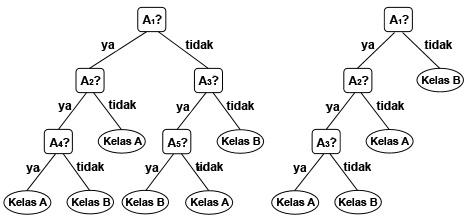
\includegraphics[scale=1]{Gambar/treepruning.jpg}
\caption[\texttt{Decision Tree Pruned}]{\texttt{Decision tree} yang belum dipotong dan yang sudah dipotong, \cite{DM}} 
\label{fig:treePruning}
\end{figure}

Terdapat dua pendekatan dalam melakukan \textsl{pruning}, yaitu \textsl{prepruning} dan \textsl{postpruning}.

Pada \textsl{prepruning}, pemotongan pohon dilakukan dengan cara menahan dan tidak melanjutkan pembuatan cabang atau partisi dari sebuah node, dan membuat node tersebut menjadi \textsl{leaf}. 

Pada \textsl{postpruning}, pemotongan pohon dilakukan ketika \textsl{decision tree} sudah selesai dibangun dengan cara menggubah cabang pohon menjadi \textsl{leaf}.

\subsection{\textsl{Pattern Evaluation}}
\textsl{Pattern evaluation} merupakan tahap mengidentifikasi apakah \textsl{pattern} atau pola tersebut menarik dan merepresentasikan \textsl{knowledge} berdasarkan beberapa \textsl{interestingness measures}.
Suatu \textsl{pattern} atau pola dapat dinyatakan menarik apabila
\begin{itemize}
	\item mudah dimengerti oleh manusia
	\item valid untuk data percobaan maupun data yang baru
	\item memiliki potensi atau berguna
	\item merepresentasikan \textsl{knowledge}
\end{itemize}

\subsection{\textsl{Knowledge Presentation}}
\textsl{Knowledge presentation} merupakan tahap representasi dan visualisasi terhadap \textsl{knowledge} yang merupakan hasil dari \textsl{knowledge discovery}.	
%\section{\textsl{Spatial and Spatiotemporal}}

\section{Log Histori KIRI}

KIRI memiliki log histori yang melakukan pencatatan untuk setiap user ketika menggunakan KIRI. Data log tersebut diperoleh dengan cara melakukan wawancara dengan CEO KIRI, yaitu Pascal Alfadian. Data log yang diberikan sudah dalam format excel.

\textsl{Log} tersebut memiliki 5 \textsl{field} untuk setiap tuple sebagai berikut:
\begin{itemize}
	\item logId, primary key dari tuple
	\item APIKey, mengidentifikasikan sumber dari pencarian ini
	\item \textsl{Timestamp} (UTC), waktu ketika pengguna KIRI mencari rute angkot menggunakan waktu UTC / GMT
	\item \textsl{Action}, tipe dari log yang dibuat.
	\item AdditionalData, mencatat data-data yang berhubungan sesuai dengan nilai atribut\textsl{action}
\end{itemize}

LogId merupakan \textsl{field} dengan tipe data int dengan batas 6 karakter yang digunakan sebagai \textsl{primary key} dari tabel tersebut. LogId diisi dengan menggunakan fungsi \textsl{increment integer}. \textsl{Increment integer} merupakan fungsi untuk pengisian data pada database dengan menambahkan nilai 1 dari nilai yang terakhir kali diisi.
APIKey merupakan \textsl{field} dengan tipe data varchar yang digunakan untuk memeriksa pengguna KIRI ketika menggunakan KIRI.
\textsl{Timestamp} (UTC) merupakan \textsl{field} dengan tipe data \textsl{timestamp} yang digunakan untuk mencatat waktu penggunaan KIRI oleh user, diisi dengan menggunakan fungsi \textsl{current time}. \textsl{Current time} merupakan fungsi untuk pengisian data pada database dengan mengambil waktu pada komputer ketika record dibuat.
\textsl{Action} merupakan \textsl{field} dengan tipe data varchar yang digunakan untuk memeriksa fungsi apa yang dipanggil dari API KIRI. Terdapat beberapa tipe pada \textsl{field} ini, yaitu
\begin{itemize}
	\item \textsl{ADDAPIKEY}, \textsl{action} yang dicatat ke dalam log ketika fungsi pembuatan \textsl{API key} yang baru dipanggil.
	\item \textsl{FINDROUTE}, \textsl{action} yang dicatat ketika user melakukan pencarian rute
	\item \textsl{LOGIN}, \textsl{action} yang dicatat ketika developers melakukan login dengan menggunakan \textsl{API key}
	\item \textsl{NEARBYTRANSPORT}, \textsl{action} yang dicatat ketika user mencari transportasi di daerah rute sedang dicari
	\item \textsl{PAGELOAD}, \textsl{action} yang dicatat ketika user memasuki halaman KIRI
 	\item \textsl{REGISTER},\textsl{action} yang dicatat ketika developers melakukan pendaftaran pada KIRI \textsl{API key}
	\item \textsl{SEARCHPLACE}, \textsl{action} yang dicatat ketika user memanggil fungsi pencarian lokasi dengan menggunakan nama tempat
	\item \textsl{WIDGETERROR}, mencatat log tersebut ketika user menerima error dari \textit{widget}
	\item \textsl{WIDGETLOAD}, mencatat log tersebut ketika user mengdownload widget
\end{itemize}
AdditionalData, merupakan \textsl{field} dengan tipe data varchar yang digunakan untuk mencatat informasi yang dibutuhkan sesuai dengan \textsl{field action}. Isi dari additionalData tersebut untuk setiap \textsl{action} adalah
\begin{itemize}
	\item Jika nilai atribut \textsl{action} adalah \textsl{ADDAPIKEY}, maka isi nilai dari additionalData adalah nilai \textsl{API key} yang dihasilkan
	\item Jika nilai atribut \textsl{action} adalah \textsl{FINDROUTE}, maka isi nilai dari additionalData adalah \textsl{latitude} dan \textsl{longitude} lokasi awal dan tujuan serta banyak jalur yang dihasilkan dari aplikasi KIRI
	\item Jika nilai atribut \textsl{action} adalah \textsl{LOGIN}, maka isi nilai dari additionalData adalah id dari user yang melakukan login serta status apakah user berhasil login atau tidak
	\item Jika nilai atribut \textsl{action} adalah \textsl{NEARBYTRANSPORT}, maka isi dari additionalData adalah \textsl{latitude} dan \textsl{longitude} dari transportasi tersebut
	\item Jika nilai atribut \textsl{action} adalah \textsl{PAGELOAD}, maka isi nilai dari additionalData adalah ip dari user
	\item Jika nilai atribut \textsl{action} adalah \textsl{REGISTER}, maka isi nilai dari additionalData adalah alamat email yang digunakan untuk meregister dan nama user
	\item Jika nilai atribut \textsl{action} adalah \textsl{SEARCHPLACE}, maka isi nilai dari additionalData adalah nama tempat yang dicari
	\item Jika nilai atribut \textsl{action} adalah \textsl{WIDGETERROR}, maka isi nilai dari additionalData adalah isi pesan dari error yang terjadi
	\item Jika nilai atribut \textsl{action} adalah \textsl{WIDGETLOAD}, maka isi nilai dari additionalData adalah ip dari user yang melakukan download widget
\end{itemize}

\subsection{Perhitungan Nilai Jarak Menggunakan \textsl{Euclidean}}
\textsl{Euclidean} dapat menghasilkan nilai jarak antar dua objek. Misal kita memiliki dua objek (p dan q). Jika kedua objek tersebut merupakan objek dengan satu dimensi, maka rumus \textsl{euclidean} akan menjadi

\begin{displaymath}
	\sqrt{(p - q)^{2}} = |p - q|
\end{displaymath} 

Jika objek p dan q merupakan objek dua dimensi, maka rumus \textsl{euclidean} akan menjadi

\begin{displaymath}
	d(p,q) = \sqrt{(p_{1} - q_{1})^{2} + (p_{2} - q_{2})^{2}}
\end{displaymath}

Jika objek p dan q merupakan objek tiga dimensi, maka rumus \textsl{euclidean} akan menjadi

\begin{displaymath}
	d(p,q) = \sqrt{(p_{1} - q_{1})^{2} + (p_{2} - q_{2})^{2} + (p_{3} - q_{3})^{2}}
\end{displaymath}

Jika objek p dan q merupakan objek n dimensi, maka rumus \textsl{euclidean} akan menjadi

\begin{displaymath}
	d(p,q) = \sqrt{(p_{1} - q_{1})^{2} + (p_{2} - q_{2})^{2} + ..... + (p_{n-1} - q_{n-1})^{2} + (p_{n} - q_{n})^{2}}
\end{displaymath}

Contoh studi kasus untuk perhitungan dua objek dengan dimensi dua, misal terdapat dua objek dengan nilai posisi (x,y). Objek pertama terletak pada posisi 3,5 sedangkan objek kedua terletak pada posisi 4,7. Maka perhitungan jarak kedua objek tersebut adalah

\begin{displaymath}
	d(o1,o2) = \sqrt{(3 - 4)^{2} + (5 - 7)^{2}}
	d(o1,o2) = 2.236068
\end{displaymath}















